\section{The Core module}
The Core is a coordinating module which delegates the actual operation execution to other specialized modules. It controls the execution of IPOL experiments and delegates tasks such as data pre-processing (Conversion module), execution dispatching (Dispatcher module), algorithm execution (DemoRunner module), or results archiving (Archive module), among others

Figure \ref{fig:core_diagram} shows a diagram that explains the modules and the messages passed when executing an experiment. \ToDo{This need to be moved to the Sec. \ref{sec:Dispatcher}, Dispatcher}.

In order to distribute the load among several machines, the Core checks the load of each known DemoRunner (see Sec~\ref{sec:DemoRunner}) and sends the execution to a chosen demoRunner in a distant machine. It uses a FIFO queue as a ``buffer'' to wait for a computer free to execute the demo and encapsulates an object to establishes the balancing policy that decides whether a process can leave the queue or not. Finally, the core uses the selected machine and waits until the experiment is finished. When it is finished, the core send to the archive module (see Sec~\ref{sec:archive}) a JSON message for storing the experiment information.\ToDo{This should be explained in the Dispatcher and demoRunner sections}

\begin{figure}[!ht]
\centering
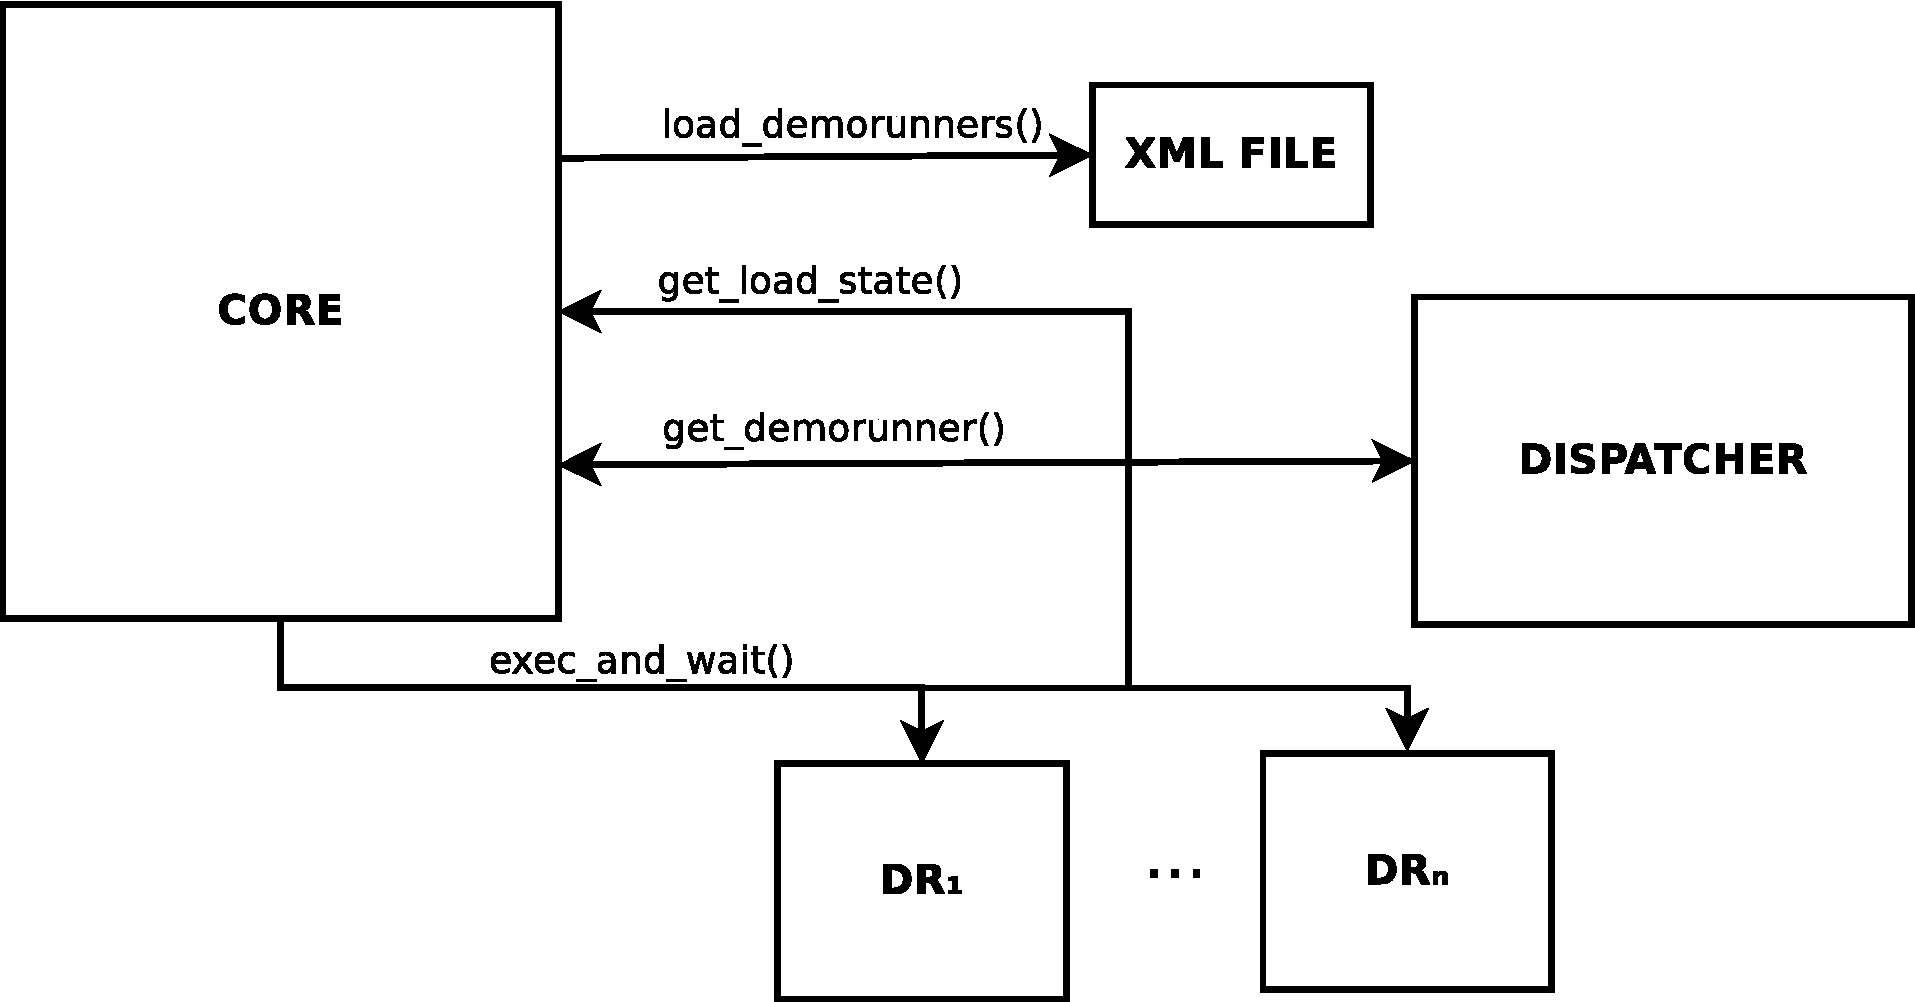
\includegraphics[width=0.7\columnwidth]{core/images/core_dispatcher.pdf}
\caption{Communication between the Core, Dispatcher, and the DemoRunner modules.}
\label{fig:core_diagram}
\end{figure}


\ToDo{Document the run program of the Core, and which are the main operations which are performed and which are delegated. For example: blob conversion, copy blobs, ask the dispatcher for the best demoRunner according to a policy chosen by the Core, send the execution to a demoRunner, delegate in Archive to store the results if needed, etc. It should also be explained the shared folder.}

\subsection{DemoExtras}

For the execution of some demos it is necessary some extra files called DemoExtras. Those files are stored in a compressed file (.tar.gz)
in the demoinfo module. Also, a copy of this compressed file is stored in the ``dl\_extras'' folder in the ``shared\_folder'' for comparison
reasons.

The first time a DemoExtra is found, the core uncompress the file into ``DemoExtras'' folder in the ``shared\_folder''. And in each execution
the core checks the date and the size of the compressed file in the ``shared\_folder'' with the one stored in demoinfo.

The possible results from the check are:
\begin{itemize}
 \item \textbf{Date and size match:} Nothing is done
 \item \textbf{Date or size don't match:} The DemoExtra is downloaded again
 \item \textbf{DemoExtra deleted in demoinfo:} All DemoExtras files related to that demo are deleted in the ``share\_folder''
\end{itemize}

